\documentclass[a4paper, 10pt, final, garamond]{book}
\usepackage{cours-preambule}

\titleformat{\item}{}{\arabic{item})}{.5em}{}{}
\titleformat{\subitem}{}{\arabic{item}) \alph{subitem} --}{.5em}
{}{}

\makeatletter
\renewcommand{\@chapapp}{Devoir maison -- chapitre}
\makeatother

\begin{document}
\setcounter{chapter}{0}

\chapter{Commentaires sur le DM}

\begin{NCprop}[width=\linewidth]{\centering\bfseries\ Malus}
    Chacune des lettres suivantes sur vos copies sont des malus de \num{0.25}
    points.\smallbreak
    \begin{minipage}{0.50\linewidth}
        \begin{itemize}
            \item A~: application numérique (mélange littéral numérique)~;
            \item N~: numéro de copie~;
            \item P~: prénom sur copies~;
            \item E~: encadrement des réponses~;
            \item M~: marge non laissée ou trop grande~;
            \item D~: doublon avec une autre copie~;
        \end{itemize}
    \end{minipage}
    \begin{minipage}{0.50\linewidth}
        \begin{itemize}
            \item Q~: numéro de question mal ou non indiqué (même passées)~;
            \item C~: copie grand carreaux~;
            \item R~: respect~;
            \item U~: valeur numérique sans unité~;
            \item H~: homogénéité non respectée~;
            \item S~: chiffres significatifs non cohérents.
        \end{itemize}
    \end{minipage}
\end{NCprop}

\section{Commentaires généraux}
\begin{center}
    \Huge Un devoir maison se traite entièrement
\end{center}

C'est une honte de voir tant de copies traiter si peu de questions en
\textbf{deux semaines}. 6 points sur les 3 premières questions, avec des
exercices vus en cours (fibre, mirage), c'est illégal d'avoir moins que 6 au
total. Vous n'êtes plus au lycée, il est temps de vous réveiller. Vous devez
venir ici en tant que scientifiques en devenir et avec la volonté de devenir des
expert-es, pas pour faire plaisir à vos parents.

Aucun respect pour les commentaires sur le premier DM rendus le 15/09. Trop de
schémas manquant pour introduire les notations. Vous ne savez pas lire des
énoncés~: une question peut comporter plusieurs sous-questions. «~Commenter~»
n'est pas une question en l'air. Donc \textbf{soulignez chaque sous-question
dans une question et barrez-la quand répondue}.

Si vous sautez des questions, \textbf{Écrivez les numéros des questions non
traitées}. Et si vous recopiez sur votre camarade, \textbf{rendez une seule
copie pour plusieurs personnes !! Malus associé.}

\section{Exercice I \hfill \textcolor{red}{/3}}

\begin{enumerate}
    \item{C'était le cours. Flèche oubliée, plan d'incidence oublié = moitié des
        points. \hfill \textcolor{ForestGreen}{/1}}

    \item{Le laser est perpendiculaire au dioptre sphérique~: «~suivant un de
            ses rayons~». Schémas aléatoires, vous ne savez pas tracer des
            normales à un dioptre. On vérifie SD, la \textit{réflexion totale},
            et laser monochromatique et un seul angle d'incidence. \textbf{Lisez
            bien toute la question pour ne pas oublier des parties !}\hfill
        \textcolor{ForestGreen}{/2}}
\end{enumerate}

\section{Exercice II\hfill \textcolor{red}{/\num{10.5}}}

\begin{enumerate}[start=3]
    \item{C'était corrigé en TD. \textbf{Si vous inventez une notation, faites
            un schéma !!}. Il fallait mentionner la réflexion totale. Réponse
            avec 4CS. Les $n\times c$ à la place de $n_c$ sont choquants, et
            leur apparition dans plusieurs copies montre un recopiage
        honteux. Un schéma avec un rayon entrant qui s'écarte de la normale est
    faux, cf.\ corrigé TD2.\hfill \textcolor{ForestGreen}{/3}}

    \item{Ok\hfill \textcolor{ForestGreen}{/.5}}
    \item{Quelques bons schémas, sinon aucun explication pour la détermination
            de la plus grande distance. Pas de magie noire en sciences.\hfill
        \textcolor{ForestGreen}{/1}}
    \item{Simple différence. Moitié des points si cohérence avec question
            précédente. Moitié des points si expression donnée sous une forme
        trop laide.\hfill \textcolor{ForestGreen}{/.5}}
    \item{\textbf{Lisez l'énoncé !!} Il fallait utiliser les expressions données
        et calculer $\delta T$, pas $\Delta$.}
    \item{Il fallait une amplitude plus faible et un étalage plus grand. Les
            axes s'orientent et prennent un label.\hfill
        \textcolor{ForestGreen}{/.5}}
    \item{Peu de compréhension sur cette question, en tout cas peu de
            justification. Les signaux se recouvrent si la période entre deux
            impulsions est plus petite que l'étalage du signal (faire
        schéma).\hfill \textcolor{ForestGreen}{/.5}}
    \item{Globalement ok, mais que peu de réponses correctes sur l'intérêt~:
        grandeur uniquement liée aux caractéristiques de la fibre.\hfill
    \textcolor{ForestGreen}{/1}}
    \item Manque de compréhension aussi~: \textit{bits} reliés à $f$, pas $B_0$.
        Vous ne réfléchissez pas à ce que vous faites, c'est écrit dans la
        question 9. 3CS\hfill \textcolor{ForestGreen}{/.5}
    \item Trop de personnes pensent que la réflexion totale est à éviter. C'est
        tellement aberrant dans cet exercice j'en suis abasourdie. C'est tout
        l'inverse, avec une courbure on peut perdre la réflexion totale.\hfill
        \textcolor{ForestGreen}{/.5}
    \item Sans schéma il est impossible de répondre correctement à cette
        question. Trop de recopiage ici, avec exactement les mêmes erreurs qui
        se compensent, les $r_c-n_g$ qui redeviennent $r_c\times n_g$ subitement
        ou le $r_c$ qui se transforme en $2r_c$ comme par magie. 2CS\hfill
        \textcolor{ForestGreen}{/1}
\end{enumerate}

\begin{center}
    \Huge N'arrêtez pas un DM au milieu !!
\end{center}

\section{Exercice 3\hfill \textcolor{red}{/6.5}}
\begin{enumerate}[start=14]
    \item Honnêtement… je ne pensais pas qu'on pouvait mal répondre à cette
        question. Il suffisait d'entrer la formule dans sa calculatrice.
        \textbf{Les axes sont orientés}. \textbf{Ils ont un label}. L'axe des
        ordonnées est bien $n^2$. \textbf{Ne graduez pas vos axes verticaux de
        -1 à 1 si les valeurs sont entre \num{2.21} et \num{2.25}}. En enfin,
        \textbf{zoomez sur votre calculatrice plutôt que de me tracer quelque
        chose de plat !!} Sinon allez sur Wolfram Alpha.\hfill
        \textcolor{ForestGreen}{/.5}
    \item Ok. Dire constante.\hfill \textcolor{ForestGreen}{/.5}
    \item Il ne fallait pas se perdre en calculs, $n(y)\cos(\phi)$ était
        constante et on l'avait en $0$.\hfill \textcolor{ForestGreen}{/.5}
    \item Globalement ok.\hfill \textcolor{ForestGreen}{/1}
    \item Si l'énoncé les appelle $A_1$ et $A_2$, vous les appelez pareil~!
        Soyez malin-es, vous veniez de donner $\dv{y}{x} = \tan(\f)$ et on vous
        demande maintenant $y'(x=0)$… c'était forcément $\tan(\theta_0)$.\hfill
        \textcolor{ForestGreen}{/1}
    \item Globalement ok même si recopiage transforme des $r_c$ en $n_c$. La
        période $\lambda$, et la fonction s'annule chaque demi-période.\hfill
        \textcolor{ForestGreen}{/1}.
    \item C'était gratuit, la figure était donnée au début de l'exercice. Il
        suffisait de montrer qui était $d$ et dire que l'amplitude devait être
        plus petite que le rayon du câble…\hfill \textcolor{ForestGreen}{/.5}
    \item C'était la même O.N.\hfill \textcolor{ForestGreen}{/.5}
    \item Application numérique~: 2CS sur $\delta T'$. Commenter et interpréter
        physiquement ne sont pas optionnels.\hfill \textcolor{ForestGreen}{/1}
\end{enumerate}

\vfill

\begin{center}
    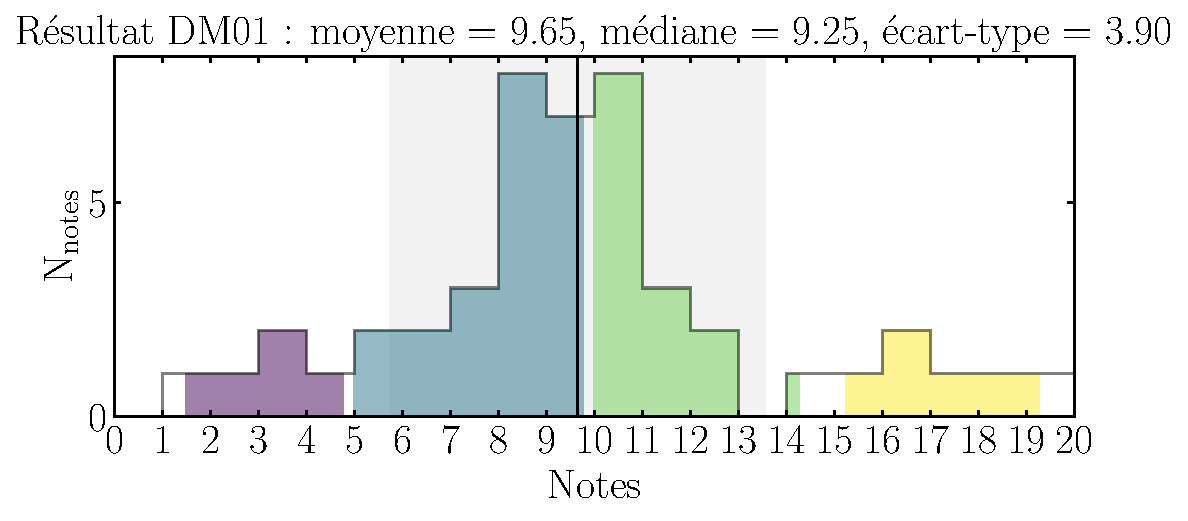
\includegraphics[width=\linewidth]{res_dm01.pdf}
\end{center}

\vfill

\end{document}

